\chapter{Experimentación y Resultados}
\section{Infraestructura utilizada}

\subsection{Simulación de Red}

En un principio se hicieron experimentos utilizando software 
de simulación de redes para poder lograr tamaños de 
\emph{anonymity-set} aceptables. Este software utilizado fue 
\emph{CORE}\footnote{\url{https://www.nrl.navy.mil/itd/ncs/products/core}} 
el cual permite emular distintos nodos en una red simulada 
con los parámetros que el usuario estime convenientes. Utilizando 
este software se simularon nodos conectados a través de una red local, 
donde cada uno de los nodos se comporta como un participante dentro 
del protocolo anteriormente descrito.

Además de dicho software, se levantaron instancias de 
\emph{Docker}\footnote{\url{https://www.docker.com/}}, pudiendo así 
formar una red local entre los distintos contenedores corriendo 
en una misma máquina.

Ambas simulaciones mostraron un pobre rendimiento a la hora de 
correr el protocolo, mostrando tiempos de un orden de magnitud 
mayores que los tiempos reales que se lograron \emph{a posteriori}.

\subsection{Uso de red real}

Luego de notar los pobres resultados obtenidos en las simulaciones, se 
pudo obtener acceso a equipos reales conectados a través de una red 
local. En particular se utilizó el laboratorio \emph{Lorenzo} del 
Departamento de Ciencias de la Computación de la Universidad de Chile, el 
cual cuenta con 31 computadores, cantidad razonable para poder realizar 
las pruebas correspondientes.

\section{Experimentos Realizados}

Las pruebas realizadas fueron dos:

\begin{enumerate}
	\item Tamaño de sala variable, todos los participantes enviando: se 
	varió el tamaño de la sala desde 3 hasta 30 participantes, donde en 
	cada repetición, todos los participantes presentes envían un 
	mensaje de largo 140 caracteres.
	\item Tamaño de sala fijo, algunos participantes enviando: se fijó 
	el tamaño de la sala en 30 participantes, y en cada repetición se 
	aumentaba el número de mensajes (cada uno de 140 caracteres) enviados, 
	desde 1 hasta 30.
\end{enumerate}

En cada una de las dos pruebas realizadas se midieron los siguientes 
parámetros:

\begin{itemize}
	\item Tiempos de ejecución: se midieron tres distintos tiempos, (1) tiempo 
	total de ejecución, (2) tiempo que demora en llegar el primer mensaje, y 
	(3) tiempo promedio por ronda.
	\item \emph{Profiling} de cada etapa del protocolo: se midió que porcentaje 
	del tiempo total se gasta en cada una de las etapas del protocolo, en particular 
	cuanto tiempo se ocupa en etapas de procesamiento, y cuanto tiempo se ocupa 
	en etapas de comunicación.
	\item Ancho de banda resultante: al finalizar cada sesión, se midió el tamaño 
	total de los mensajes enviados,y se dividió por la cantidad de tiempo que 
	duró la misma sesión, obteniendo así el ancho de banda que ofrece el canal 
	anónimo implementado. 
\end{itemize}

\section{Resultados}

\subsection{Tiempos de Ejecución}

\begin{figure}[h]
  \centering
    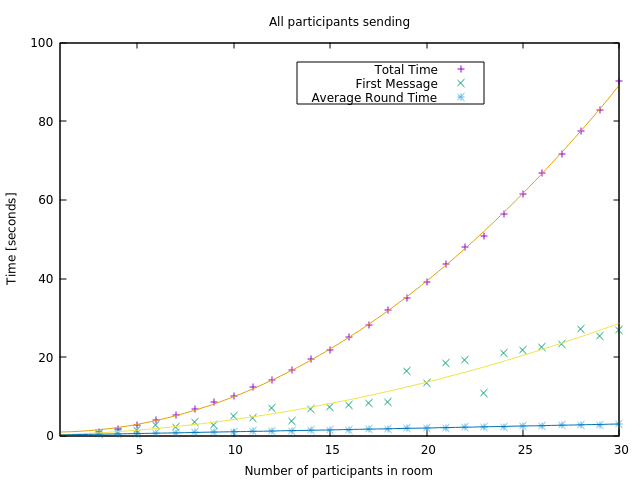
\includegraphics[scale=0.7]{logs/logs_all/times.png}
  \caption{Tiempos de Ejecución en Tamaño de sala variable}
\end{figure}

\begin{figure}[h]
  \centering
    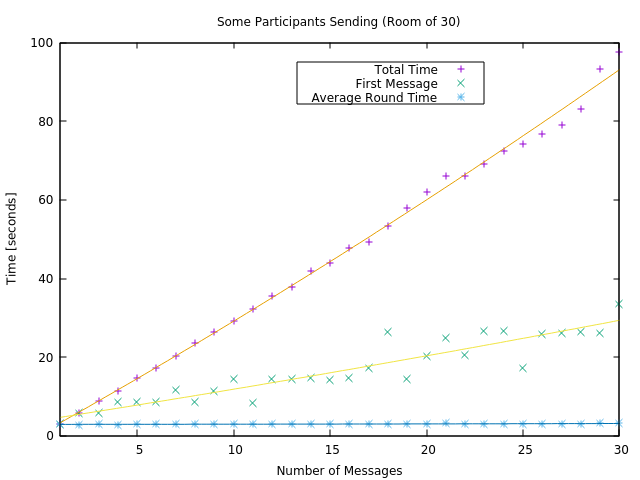
\includegraphics[scale=0.7]{logs/logs_partial_30/times.png}
  \caption{Tiempos de Ejecución en Tamaño de sala fijo}
\end{figure}

\subsection{\emph{Profiling} de las etapas}

\begin{figure}[h]
  \centering
    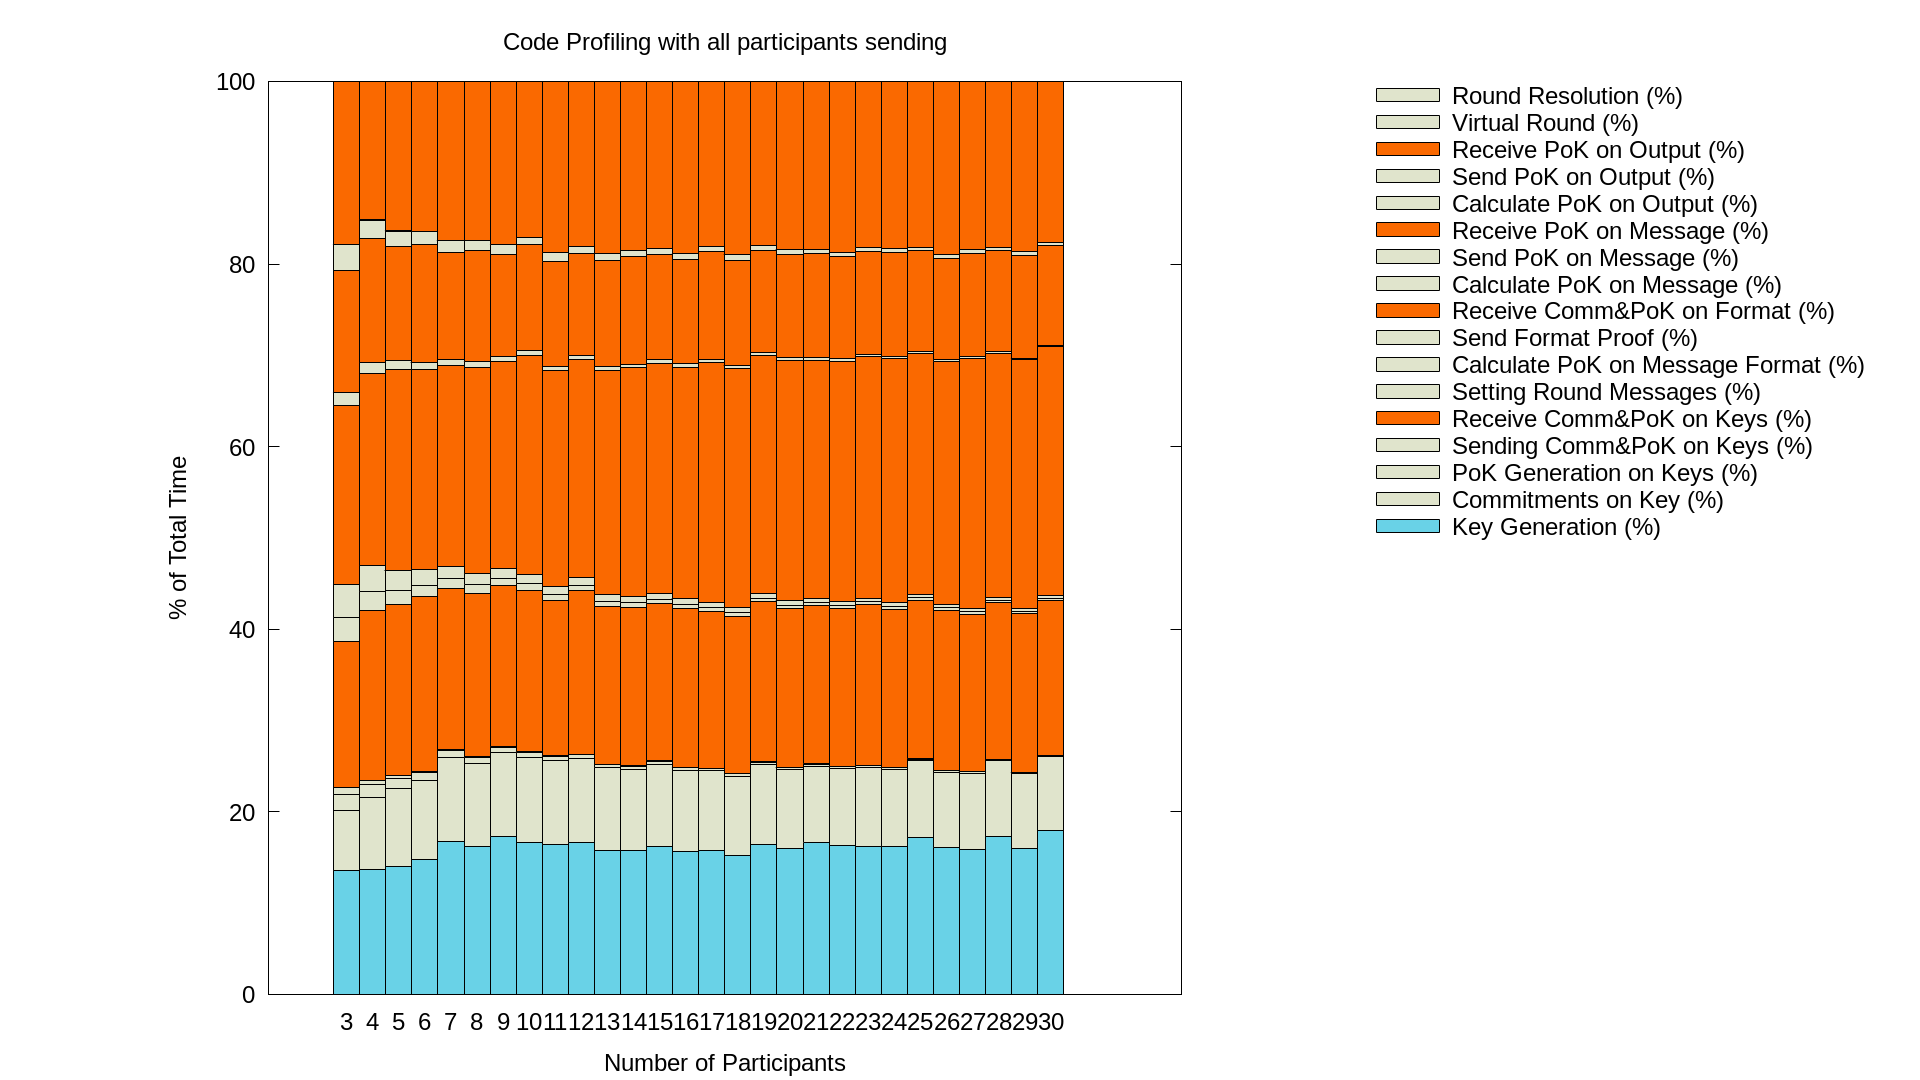
\includegraphics[scale=0.3]{logs/logs_all/profile.png}
  \caption{\emph{Profiling} de etapas en Tamaño de sala variable}
\end{figure}

\begin{figure}[h]
  \centering
    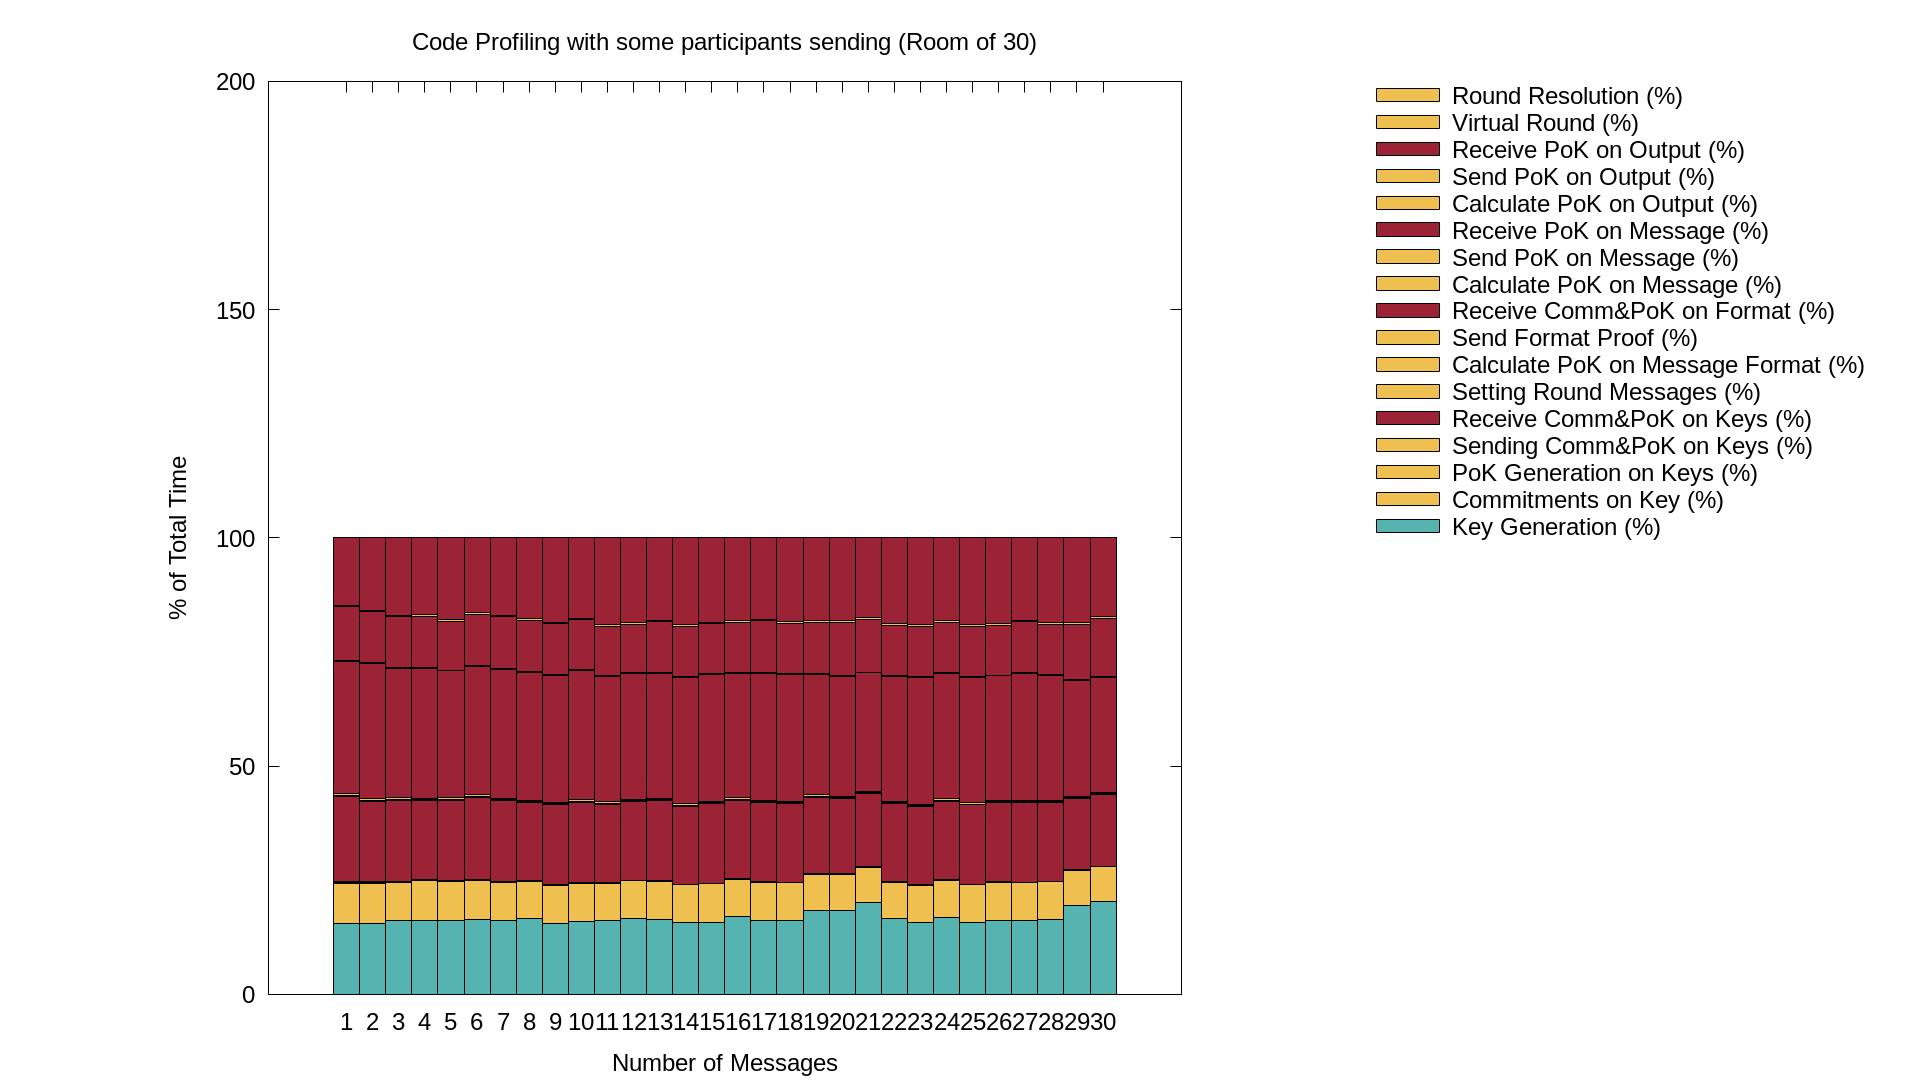
\includegraphics[scale=0.3]{logs/logs_partial_30/profile.png}
  \caption{\emph{Profiling} de etapas en Tamaño de sala fijo}
\end{figure}

\subsection{Ancho de banda}

\section{Discusión de los Resultados}